\documentclass[11pt]{article}
\usepackage{hyperref}
\usepackage{graphicx}
\usepackage[margin=1in]{geometry}
\usepackage{subcaption}
\usepackage{xcolor}
\usepackage{listings}

\bibliographystyle{ieeetr} 


\definecolor{mygreen}{rgb}{0,0.6,0}
\definecolor{mygray}{rgb}{0.5,0.5,0.5}
\definecolor{mymauve}{rgb}{0.58,0,0.82}

\lstset{ %
  backgroundcolor=\color{white},   % choose the background color; you must add \usepackage{color} or \usepackage{xcolor}
  basicstyle=\footnotesize,        % the size of the fonts that are used for the code
  breakatwhitespace=false,         % sets if automatic breaks should only happen at whitespace
  breaklines=true,                 % sets automatic line breaking
  captionpos=b,                    % sets the caption-position to bottom
  commentstyle=\color{mygreen},    % comment style
  deletekeywords={...},            % if you want to delete keywords from the given language
  escapeinside={\%*}{*)},          % if you want to add LaTeX within your code
  extendedchars=true,              % lets you use non-ASCII characters; for 8-bits encodings only, does not work with UTF-8
  frame=single,	                   % adds a frame around the code
  keepspaces=true,                 % keeps spaces in text, useful for keeping indentation of code (possibly needs columns=flexible)
  keywordstyle=\color{blue},       % keyword style
  language=Octave,                 % the language of the code
  otherkeywords={*,...},           % if you want to add more keywords to the set
  numbers=left,                    % where to put the line-numbers; possible values are (none, left, right)
  numbersep=5pt,                   % how far the line-numbers are from the code
  numberstyle=\tiny\color{mygray}, % the style that is used for the line-numbers
  rulecolor=\color{black},         % if not set, the frame-color may be changed on line-breaks within not-black text (e.g. comments (green here))
  showspaces=false,                % show spaces everywhere adding particular underscores; it overrides 'showstringspaces'
  showstringspaces=false,          % underline spaces within strings only
  showtabs=false,                  % show tabs within strings adding particular underscores
  stepnumber=2,                    % the step between two line-numbers. If it's 1, each line will be numbered
  stringstyle=\color{mymauve},     % string literal style
  tabsize=2,	                   % sets default tabsize to 2 spaces
  title=\lstname                   % show the filename of files included with \lstinputlisting; also try caption instead of title
}
\begin{document}


\title{Classification of bird species based on recorded bird-bird-soundsounds}
\author{Pritam Sukumar}
\date{\today}
\maketitle

\tableofcontents


\section{Definition}

A friend and I are building an app that will use machine learning to recognise bird sounds from iPhone recordings, and I wanted to use this project as an opportunity to explore work that has already been done in this area. While researching potential topics related to bird sound recognition, I found a Kaggle competition \hyperref{https://www.kaggle.com/c/mlsp-2013-birds}{MLSP 2013 Bird Classification Challenge} that deals with the same exact problem along with a potential approach that I could try out. I decided to go along with the steps and implement the machine learning portions of the competition myself to learn more about this field.

\subsection{Project Overview}

The recognition of bird sounds holds importance for a variety of reasons. Identifying the bird species in a given region allows scientists to prepare surveys of current populations, along with aiding studies of specific species, investigating the effect of environmental factors such as climate change, and also providing data for making predictions about the future in that area. Also, the hobby of bird watching has grown immensely, and for bird watchers, spotting a new species (or even a known one) is a very pleasing experience.

Identifying birds present in an area for scientific research is an expensive task, both in terms of time and money, due to the necessity of in-the-field researchers. For hobbyists, it has always been a challenge -- and, to be honest, part of the charm -- to recognise new species in the wild. In recent years,  there has been a strong interest in the possibility of using machine learning for this task. 

One approach that was followed (and is explored in this project), is using data from microphones placed in the forest. This has the advantage of not needing human presence to record the sounds. The microphones are retrieved every few weeks and the data is used to identify the bird species present in the recording. In this project, I am going to try to (or rather verify) that it is indeed practical, and that the accuracy that we can obtain using relatively new data-processing and machine learning techniques is very promising for the future of bird-sound recognition and my app.

\subsection{Problem Statement}

The scope of this project is defined by the scope of the \hyperref{https://www.kaggle.com/c/mlsp-2013-birds}{Kaggle competition}. The task is to use machine learning to automatically detect the species of bird in a recording made in the wild. The recordings are usually of short duration. However, they may contain no birds (as is the case for most of the day), or multiple birds in the same recording (as is often the case for recordings taken at dawn or dusk). 

The strategy applied for this task is to understand how to extract information from the sound recordings. This usually entails the following steps:

\begin{enumerate}
\item Detecting whether bird sounds exist in the wave file
\item Separating the bird sounds from the background noise (streams, rain, etc.)
\item Detecting whether there are one more more birds
\item Separating the individual bird sounds 
\item Processing the bird sounds in a way that is friendly to machine learning classification
\end{enumerate}

I intend to retrace the steps of a paper that accompanies the Kaggle competition. The first step is generating a spectrogram, i.e. converting the audio file to the frequency domain because birds vary much more by pitch than by amplitude (which is what a usual wave file will provide). Once that is done, we reduce the noise in the data, and then separate out the bird sounds from the rest of the audio (the segmentation problem), and also from each other (the cocktail party problem). 

Then we can run a classifier over the segmented frequency graphs to detect the birds in a given recording. Note that the problem complexity increases because this a Multi-Instance Multi-Label (MIML) problem, i.e. Every audio file can have multiple bird sounds (instances) in it, and each instance of a bird sound can correspond to one of many different birds (labels). 

In this project, I try four different classifiers to compare their performance: Decision Trees, K-nearest neighbours, Random Forest Regressors, and Logistic Regression. The working of these algorithms is briefly explained in Section \ref{sec-algorithms}.

The final result should be something along the lines of: ``In recording $m$, there are three birds present, which are $x,y,$ and $z$."

\subsection{Metrics}

Since I am using a dataset from an expired Kaggle competition, the metrics are defined by the rules of the competition. In this case, the metric is the overall accuracy of the classification as measured by the area under the ROC curve. As defined by the competition, the ROC curve is generated by taking as input the labels generated by the algorithm, along with the predictions.

The ROC (Receiver Operating Curve) is a curve that plots the true positive rate versus the false positive rate for a binary classification algorithm. The AUC (Area Under the Curve) represents the accuracy of the algorithm.

In the case of the bird-classification problem, since the problem is multiclass, we need to first convert it to a binary classification problem. We do this by simply treating the presence of each bird in each recording as a separate instance for the algorithm. This way, every sound recording corresponds to nineteen classifications.

Reframing the problem as a binary problem (Binary Relevance) has the disadvantage of biasing the accuracy metric towards true negatives, since there is a higher probability that a bird will not be present in most of the recordings. Since the ROC curve is plotting the true positive rate versus the false positive rate, each point on the ROC plot effectively represents \textit{two} instances, one each from the correct and incorrect classification groups. Thus, if every example were marked as absent, the AUC would be 0.5. 

\section{Analysis}

In this section, I present an analysis of the specific problem at hand, including a description of the dataset, the approach followed to solve the problem, an explanation of how the audio recognition problem is transformed into an image recognition problem, and finally, the specific machine learning techniques I tried to use for this problem, along with reasoning for them.

\subsection{Data exploration}

The training set consists of 323 wave files, representing sounds from 19 species of birds (see Table \ref{bird_name_table}). Each recording contains up to 7 species of birds making sounds in them, maybe simultaneously.

\begin{table}[h]
\centering
\caption{Birds present in the dataset}
\label{bird_name_table}
\begin{tabular}{|l|l|l|}
\hline
Code & Name                       \\ \hline\hline
0    & Brown Creeper              \\ \hline
1    & Pacific Wren                \\ \hline
2    & Pacific-slope Flycatcher    \\ \hline
3    & Red-breasted Nuthatch       \\ \hline
4    & Dark-eyed Junco             \\ \hline
5    & Olive-sided Flycatcher      \\ \hline
6    & Hermit Thrush               \\ \hline
7    & Chestnut-backed Chickadee   \\ \hline
8    & Varied Thrush              \\ \hline
9    & Hermit Warbler              \\ \hline
10   & Swainson's Thrush           \\ \hline
11   & Hammond's Flycatcher        \\ \hline
12   & Western Tanager             \\ \hline
13   & Black-headed Grosbeak       \\ \hline
14   & Golden Crowned Kinglet      \\ \hline
15   & Warbling Vireo              \\ \hline
16   & MacGillivray's Warbler      \\ \hline
17   & Stellar's Jay               \\ \hline
18   & Common Nighthawk            \\ \hline
\end{tabular}
\end{table}

The dataset is quite unbalanced with respect to each of the species, as shown in Figure \ref{bird_species_count}. In the region where the recordings were made, it looks like Swainson's Thrush was pretty common (more than 60 examples), while many other birds are represented by less than 10 recordings. This means we need an algorithm capable of handling this kind of unbalanced dataset for a multiclass problem. 

\begin{figure}[h]
\begin{center}
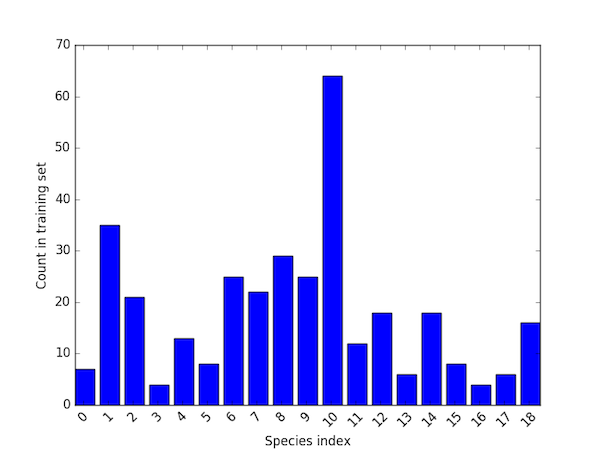
\includegraphics[width=1.0\textwidth]{../species_count_histogram.png}
\caption{Number of examples in training set for each bird species}
\label{bird_species_count}
\end{center}
\end{figure}

\subsection{Exploratory Visualization}

As mentioned briefly in the preceding section, each recording can contain more than one recording, or even none. The presence of multiple birds in the same recording presents great challenges in terms of segmentation and source separation (the so-called cocktail party problem). The presence of more than one bird-sound with the possibility for overlap indicates that we will have to do some processing to the recordings to be able to separate the bird-sounds from each other.

\subsection{Algorithm and Techniques}

To automatically classify bird-sounds, the sound recording needs to be converted to a form that is suitable as input to a machine learning algorithm. We first need to separate the bird sounds from the noise. There are two approaches commonly used to do this. Both of them rely on first extracting the spectrogram of the audio from the audio file. 

In this section, I will first discuss how the authors of the paper obtain the spectrogram, following which I will discuss the machine learning algorithms I chose to study in addition to the ones used in the research paper.

\subsubsection{Spectrograms and audio recognition}

A spectrogram is a visual representation of the frequencies present in an audio file. In the spectrograms considered in this paper, the X-axis represents time and the Y-axis represents the frequency. A point \textit{(x,y)}, represents the amplitude of frequency $y$ at time $x$. The amplitude is usually represented by a shade of white ranging from $0$ (black) all the way to $255$ (white). Black indicates that the frequency is not present at that time, and white indicates that the frequency is present at high amplitude (i.e. loud) at that point of time, with shades in between filling in the range.

\begin{figure}
\begin{center}

\begin{subfigure}[b]{1.0\textwidth}
\includegraphics[width=1.0\textwidth]{/Users/pritamps/Dropbox/birdsong/mlsp_contest_dataset/spectrograms/PC1_20090606_070012_0040.bmp}
\caption{Example Spectrogram}
\label{example_spectrogram}
\end{subfigure}

\begin{subfigure}[b]{1.0\textwidth}
\includegraphics[width=1.0\textwidth]{/Users/pritamps/Dropbox/birdsong/mlsp_contest_dataset/segmentation_examples/PC1_20090606_070012_0040.bmp}
\caption{Spectrogram after noise reduction and segmentation}
\label{segmented_spectrogram}
\end{subfigure}

\caption{Example spectrograms provided along with the competition dataset}
\end{center}
\end{figure}

Most recognition problems (and work in many other areas) depend on a spectrogram since the frequencies present in an audio are, in fact, the things that define it. Also, using the frequencies allows us to automatically account for the effect of loudness since the frequency does not depend on loudness.

For sound recognition, there are two approaches that are popular:

\begin{enumerate}
\item Get a vector descriptive of the frequency range in the spectrogram and use that for recognition. One way to do this is convert the spectrogram to a \textit{Mel-Spectrum}, i.e. apply a bunch of filters spaced logarithmically over the range of human frequencies to get a set of vectors for each of the syllables and/or sounds present in the audio. The vector can then be used as an input to a Machine Learning algorithm.
\item Use the spectrogram as an input to an image recognition problem, thus enabling the use of techniques such as segmentation and histogram-of-gradients. We can separate out sounds using segmentations and then each sound can be fed into a machine learning algorithm for classification.
\end{enumerate}

\subsubsection{Generating features from the segments}

The approach followed by the Kaggle competition organisers to generate recording-wise features follows closely the approach outlined in the 2012 paper by Briggs et. al.\cite{briggs-2012}. Of the two approaches outlined above, the authors followed the second approach, i.e. using the spectrogram as input to an image recognition problems. The steps in the process are:

\begin{enumerate}
\item \textit{Noise Reduction}
\item \textit{Segmentation}: Once the spectrogram is generated, a segmentation algorithm is run on the audio files to separate the individual bird sounds from the audio. The segmentation algorithm is trained using 20 of the wave files that have been manually segmented by humans, and then a Random Forest is used on the rest of the data to separate the segments. 

An example spectrogram of a recording and the result after noise reduction segmentation on the same recording are provided in Figures \ref{example_spectrogram} and \ref{segmented_spectrogram}. The red segments indicate non bird-sounds (for example, wind or trees or rivers) and the blue segments indicate a probable bird sound.

\item \textit{Segment-wise features}: After the segments are separated, a histogram-of-gradients feature is used to generate a feature vector for each of the segments. 

\item \textit{Bag-of-words feature for each recording}: Note that the number of segments in an image may vary, so applying a machine learning algorithm to the segment features directly will be cumbersome. Instead of doing that, we generate bags-of-features from the histograms. Bags-of-features (commonly called bag-of-words) is a technique commonly used in text processing that provides information with how often a particular feature occurs in an instance. 

Basically, they are a way to accumulate information from different features into a single training instance. The output is a single fixed-length feature vector that can then be used for classification in a MIML problem. The final histogram-of-gradients features are provided along with the competition dataset and are 100x1 vector, and are what I used as input to my learning algorithm.

\end{enumerate}

\subsubsection{Algorithms for classification}
\label{sec-algorithms}

It is not obvious immediately which machine learning algorithm would be most-suited to this task, so I decided to try a variety of algorithms:

\begin{enumerate}

\item Decision Trees (DTs): Decision trees reframe the classification problem as a tree, where at each node, a branch is taken based on a feature property. The properties of the tree are found using an iterative adaptive boosting algorithm, the most common of which is the AdaBoost. The advantage of decision trees are that they are partially immune to noise and the presence of outliers. However, trees are prone to overfitting, sometimes resulting in deep trees that perform well on the training set and poorly on the testing set.

\item Random Forest Regressor (RFR):  This is the algorithm used in \cite{briggs-2012}. Simply put, random forests are collections of decision trees, trained on different parts of the training set \cite{randomForests-webLink}. Each tree votes for the final class depending on its output, and hence the final classification is the mode of all the classifications provided by each of the trees. The main advantage of RFRs over simply using a decision tree is that because we are considering multiple trees, each trained on a subset of the data, and a subset of the features, there is zero possibility of overfitting. 

\item K-nearest neighbours (KNN): KNN is a popular algorithm used for classification problems. The final classification is obtained by finding the $k$ nearest neighbours from the training examples, as measured by finding the ``distance'' between features, where distance can be arbitrarily defined, but is usually taken to be the euclidean distance. Once the $k$ nearest neighbours are found, the final classification is again taken to be the mode of the classes of the training examples.

\item Logistic Regression (LR): Logistic regression was designed to only apply to single class classification problems. However, it can easily by extended to multi-class problems. If there $n$ classes, $n$ sets of regression coefficients are found based on the training data. This is effectively the same as finding $n$ separate LRs. Thus, when a test data point is encountered, the multiclass LR outputs a separate probability for each of the classes. The sum of these probabilities is $1$, since the test data point is assumed to belong to one and only one of the classes. The predicted class is then, the class that has the maximum probability.

\end{enumerate}


\subsection{Benchmark}

If we do not use any machine learning, and instead predict that there are no birds in any of the audio files, or predict the presence or absence perfectly at random, the area under the ROC curve will be \textbf{0.5}.

The benchmark for this project was the score provided by the organisers of the competition: \textbf{0.85576}. This score is generated by treating each recording as a collection of multiple single-label classification problems. A \textbf{Random Forest} is used on the bag-of-words features to generate this score. Once the presence of each species in each recording is predicted, this is used to generate an Receiver Operating Characteristic (ROC) curve. The ROC curve is a plot of the true positive rate versus the false positive rate for the algorithm. The benchmark score is generated by measuring the area under the ROC curve. 

The goal of this project, since I am using the same features as the paper, is to meet this benchmark by using Random Forests, and to compare this with other machine learning algorithms to see if there is any difference. 

\section{Methodology}

\subsection{Data preprocessing}

No preprocessing was needed as the complex transformations from the raw audio files to the filtered spectrograms was provided by the organisers of the competition. The feature vectors were extracted from the raw text files and then split into test and training sets. The code for this can be found in \texttt{data\_extract.py}.

\subsection{Implementation}
\label{sec-implementation}

I have outlined the algorithms I tried in Section \ref{sec-algorithms}. Using the bag-of-words features provided with the dataset, I performed the classification by implementing these algorithms using the corresponding \texttt{sklearn} packages. Some of the challenges I faced were:

\begin{enumerate}
\item \textit{Converting the multiclass features to a binary relevance problem}: The features as given, each correspond to multiple bird recordings. To treat the problem as a binary relevance problem, these need to be converted to a binary problem, i.e. for each recording, instead of saying: \textit{Species (1, 5, 6) are present}, we need to say \textit{Species 1 is present, Species 2 is absent, ...,} and so on. After spending many hours in this, I found that \texttt{sklearn} supports this out of the box with a package called \textbf{MultiLabelBinarizer}. The code for extraction is included in Listing \ref{lst-extract}

\item \textit{Performing the classifications}: I wanted to try multiple algorithms with multiple sets of parameters. However, the scoring was manual, since all the scoring was done through the Kaggle scoreboard. To get around this, I created a dictionary of \textit{classifers} and then looped through them, fitting on the training data and classifying on the testing data. The results were stored at runtime in separate \texttt{csv} files which could then be uploaded to Kaggle. The code for classification is shown in Listing \ref{lst-classify}. Lines 11-37 set up the classifiers.

\item \textit{Performing the grid search}: \texttt{sklearn} includes a method to perform grid search. However, the grid search does not automatically support multiple grid values. Hence, I simply manually performed the grid search, by defining nine separate RFR classifiers. The parameters were chosen to explore ranges around the parameters chosen by the authors of the paper this work is based on. \cite{briggs-2012}. Lines 11-33 of Listing \ref{lst-classify} show the nine different classifiers used to perform the grid search.

\end{enumerate}


\subsubsection{Parameters}

To start with, the default parameters were used for each of the algorithms For the sake of completeness, they are described below:

\begin{enumerate}
\item Decision Trees: The \texttt{sklearn} implementation of DTs includes many parameters to tune \cite{dt-documentation}. The most important ones are:

\begin{enumerate}
\item \textit{Criterion}: The measure that is used to decide on which branch to take at each node. The \texttt{sklearn} DT package supports Gini impurity and entropy. The Gini entropy is used in this section
\item \textit{Maximum features}: The maximum number of features to consider in the tree. This parameter is usually modified in order to minimize overfitting. For our purposes, we leave this value at the default value, which is to use all the features.
\item \textit{Maximum depth}: The depth at which to stop growth of the tree. We do not set this value, which allows the tree to grow until all the final leaves are classes.
\end{enumerate}

\item Random Forest Regressors: The \texttt{sklearn} documentation for RFRs \cite{rfr-documentation} includes the following parameters (in addition to others) to tune:
\begin{enumerate}
\item \textit{Number of estimators}: The number of decision trees constructed by the algorithm.
\item \textit{Maximum features}: The number of features to consider when making a split at each node of each tree.
\item \textit{Random state}: The seed for the random number generator used by the algorithm.
\item \textit{DT parameters}: Parameters that are passed to the individual trees; these parameters are the same as those used by DTs.
\end{enumerate}

\item K-nearest neighbours: The \texttt{sklearn} documentation for KNNs \cite{knn-documentation} includes the following parameters to tune:

\begin{enumerate}
\item \textit{Number of neighbours}: The number of neighbours to consider for the final classification. The final classification will be the mean of these neighbours weighted by a function that is the next parameter. The default is set at 5, and that is the value we use for our analysis.
\item \textit{Weight}: The weight to give each of the $k$ neighbours. The examples can be weighted by distance from the centroid, uniformly or by a user-defined function. The default value is to use a uniform weight, i.e. to weight all $k$ neighbours equally.
\end{enumerate}

\item Logistic Regression: The \texttt{sklearn} documentation for Logistic Regression \cite{lr-documentation} tells us that the developers have kindly allowed us to change the following parameters (actually more than just these, but I am only describing the relevant ones):

\begin{enumerate}
\item \textit{Penalty}: The loss function used by the algorithm. By default the $L_2$ norm is used.
\item \textit{Multiclass formulation}: The \texttt{sklearn} LR formulations supports two ways of approaching multiclass problems: as a multinomial problem, where a joint loss function is minimized, or as a binary problem, where separate LRs are fit for each class and the final classification is the label with maximum probability. We use the binary formulation, because that is what we are using with the other algorithms as well (I discuss this again briefly in the Future work section).
\end{enumerate}

\end{enumerate}

 
 \begin{table}
 \begin{center}
\begin{tabular}{ |c|c| }
\hline
 \textbf{Algorithm} & \textbf{Score}  \\ \hline \hline
 Decision Trees & 0.66217  \\  \hline
 Logistic Regression & 0.74628 \\ \hline    
 K-nearest neighbors & 0.73433 \\ \hline
 Random Forest Regressor & 0.78726	 \\ \hline
\end{tabular}
\caption{Performance of algorithms with default parameters}
\label{tab-scores}
\end{center}
\end{table}

From Table \ref{tab-scores}, it is clear that RFRs perform the best. RFRs are also the choice of the authors of the paper the Kaggle competition was based on \cite{briggs-2012}. This is probably not a coincidence. In the next section, I report on my work on refining the RFR with the hope that the scores improve.

\subsection{Refinement}
\label{sec-refinement}

Among the algorithms, the Random Forest Regressor performed the best by far. To investigate further, I decided to investigate the performance of the algorithm with varying two parameters: the maximum number of features, and the number of estimators (trees). I performed a manual grid search (the \texttt{sklearn} grid search module does not support MIML problems) and improved the score of the algorithm. These results are tabulated in Table \ref{tab-refinement}.

The parameters that were obtained in the work of Briggs, et. al \cite{briggs-2012} are the ones in bold in the table. They are also the best combination of results. From the results of the table, it is apparent that the final score is much more sensitive to the number of estimators rather than the maximum number of features.

The cells marked ``N/A'' are those combinations of parameters for which the Kaggle scoreboard did not return a value. Unfortunately, I have no way of debugging the scoreboard, and the result files (included in the folder) look perfectly fine to me. Without the actual test labels, there is no way for me to generate the scores myself. However, I am including the parameters for completeness of the grid.

 \begin{table}
  \begin{center}
\begin{tabular}{ |c|c|c| }
\hline
 \textbf{Estimators} &  \textbf{Max. features} & \textbf{Score}  \\ \hline \hline
 10 & 16   & 0.81277 \\  \hline
 50 & 16  & N/A \\ \hline    
 100 & 16  & 0.85975 \\ \hline
 10 & 32  & 0.81287 \\ \hline
 50 & 32  & N/A \\ \hline
 \textbf{100} & \textbf{32}  & \textbf{0.86081} \\ \hline
 10 & 100  & 0.79364 \\ \hline
 50 & 100  & N/A \\ \hline
 100 & 100  & N/A \\ \hline
\end{tabular}
\caption{Grid search results on the Random Forest Regressor}
\label{tab-refinement}
\end{center}
\end{table}

\section{Results}

\subsection{Model Evaluation and Validation}

As mentioned in the Methodology section, I tried a variety of Machine Learning models to approach the problem, and found that using Random Forests exceeded the benchmark (see Section \ref{sec-implementation}). Further to that, using a manually performed grid search, I improved the performance of the algorithm (see Section \ref{sec-refinement}). A screenshot of the Kaggle results is shown in Figure \ref{kaggle_results}.

The split of training-vs-testing (50/50) and the high score on the competition leaderboard shows us that the code does generalise well to unseen data (assuming it is in a similar format). Note that the dataset already has the following issues in it, that have bean addressed while preprocessing:

\begin{enumerate}
\item Noise
\item Absence of any bird sounds
\item Multiple bird sounds
\item Overlapping bird sounds
\end{enumerate}

\subsection{Justification}

\begin{figure}[htbp]
\begin{center}
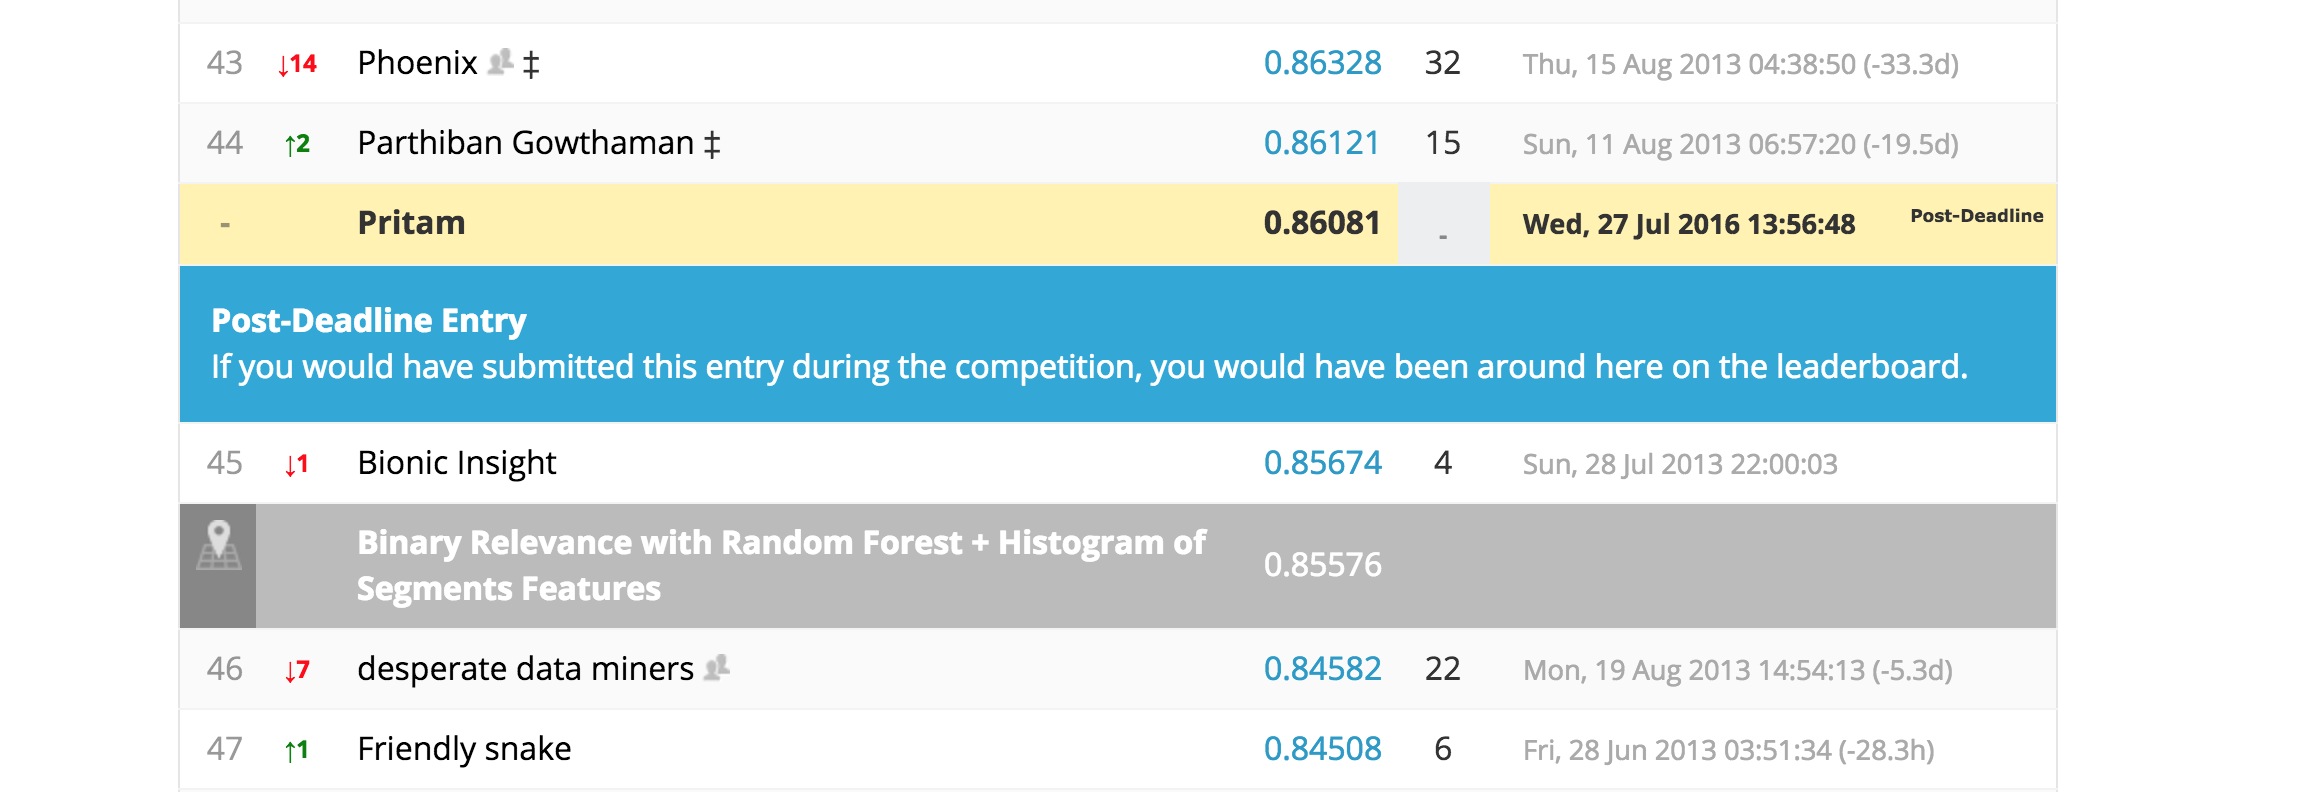
\includegraphics[width=1.0\textwidth]{../kaggle_results.png}
\caption{Best results obtained in this project}
\label{kaggle_results}
\end{center}
\end{figure}

The benchmark score was \textbf{0.85576} and my score was \textbf{0.86081}, i.e. a small improvement over the original algorithm. It is, of course, significantly better than predicting the presence of birds at random. The analysis in Section \ref{sec-refinement} justifies my final choice of parameters. 

\section{Conclusion}

\subsection{Free-form visualisation}
For the free-form visualization, I am including here a histogram of the number of species present in each recording is shown in Figure \ref{bird_species_histogram}. The histogram is particularly interesting because it shows the high percentage of recordings with \textbf{no birds} present in them.

Most of the recordings have only none or one species present in them. The high percentage of recordings with no birds is a result of these microphones being placed in the wild and autonomously recording throughout the day. Bird sounds are much more common in the morning and evening, and since the microphones were not properly optimised to account for this, a large number of the recordings have no birds in them.

\begin{figure}[h]
\begin{center}
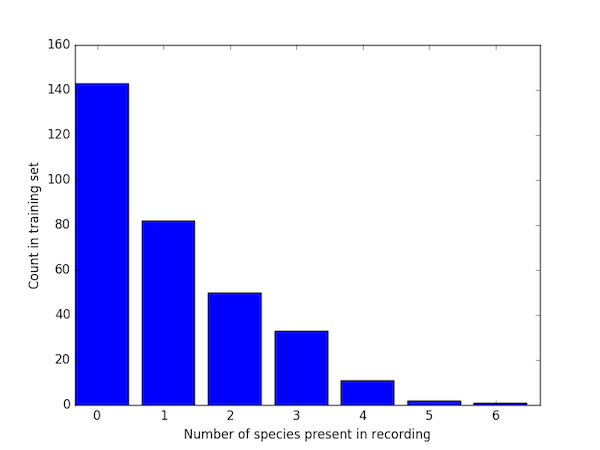
\includegraphics[width=0.75\textwidth]{../n_species_stats.png}
\caption{Histogram of number of birds in each recording}
\label{bird_species_histogram}
\end{center}
\end{figure}

\subsection{Reflection}

The problem that I attempted to solve can be summarised as follows: 

\textit{Given a recording (pre-shortened to 10 s), predict if there are any birds in the recording, and if so, how many and what species (of a subset of 20 species).}

There are many challenges in going from audio to labelling of bird species, and through this project, I intended to understand these challenges and gain experience using the tools needed to overcome them as I move to a real-world setting. These challenges include:

\begin{enumerate}
\item Noise reduction
\item Separating overlapping bird sounds (the cocktail-party problem)
\item Localising birds sounds in the audio (segmentation)
\item Solving a Multi-Instance Multi-Label (MIML) problem
\end{enumerate}

The final model as presented produced very impressive results. I am continuing to work on this topic and I hope to learn much more after finishing the MLND!

\subsection{Improvement}

One significant improvement I did not get around to implementing is including the location of the recording as an input. It is especially valid for this problem as the microphones are placed in fixed locations in the forests of Oregon. However, even in general, adding location as a variable is probably a very good idea since bird species are highly localised.

Another improvement that I do not yet have enough technical background for, is using Ensemble Classifier Chains (ECCs) instead of Binary Relevance for the MIML classifications. ECCs are known to perform much better than Binary Relevance for MIML problems, and in the future, I would love to learn more about ECCs and use them for classification.

  \begin{thebibliography}{1}

  \bibitem{briggs-2012} Forrest Briggs, Balaji Lakshminarayanan, Lawrence Neal, Xiaoli Z. Fern, and Raviv Raich {\em Acoustic classification of multiple simultaneous bird species: A multi-instance multi-label approach}  2012.

  \bibitem{randomForests-webLink}  Leo Breiman, Adele Cutler {\em Random Forests} \\ \url{https://www.stat.berkeley.edu/~breiman/RandomForests/cc_home.htm#intro}

  \bibitem{dt-documentation} Decision tree \texttt{sklearn} documentation \\ \url{http://scikit-learn.org/stable/modules/generated/sklearn.tree.DecisionTreeClassifier.html}
  
  \bibitem{rfr-documentation} Random Forest Regressor \texttt{sklearn} documentation \\ \url{http://scikit-learn.org/stable/modules/generated/sklearn.ensemble.RandomForestRegressor.html}
  
  \bibitem{knn-documentation} Decision tree \texttt{sklearn} documentation \\ \url{http://scikit-learn.org/stable/modules/generated/sklearn.neighbors.KNeighborsClassifier.html}
  
    \bibitem{lr-documentation} Logistic Regression \texttt{sklearn} documentation \url{http://scikit-learn.org/stable/modules/generated/sklearn.linear_model.LogisticRegression.htmll}
  
  \end{thebibliography}

\section*{Appendix 1: Code Listings}

\subsection*{Classification}
\lstinputlisting[language=Python, label=lst-classify, frame=single, caption=Code for classification]{../classify.py}

\subsection*{Data extraction}
\lstinputlisting[language=Python, label=lst-extract, frame=single, caption=Code for data extraction from files]{../data_extract.py}

\end{document}


